\chapter{Estudos de caso}
\label{SectionEstudosDeCaso}
Neste capítulo, será estudado a rede de 14 barras do IEEE que pode ser encontrado em \\ \href{http://labs.ece.uw.edu/pstca/pf14/pg_tca14bus.htm}{http://labs.ece.uw.edu/pstca/pf14/pg\_tca14bus.htm}
\section{Rede de 14 barras IEEE}
\label{SectionRedePequena}
Considere a rede de 14 barras na figura \ref{FigRede4barrasLinearizado}.\\
\begin{figure}[!htb]
\caption{Rede de 14 barras IEEE}
 \centering % para centralizarmos a figura
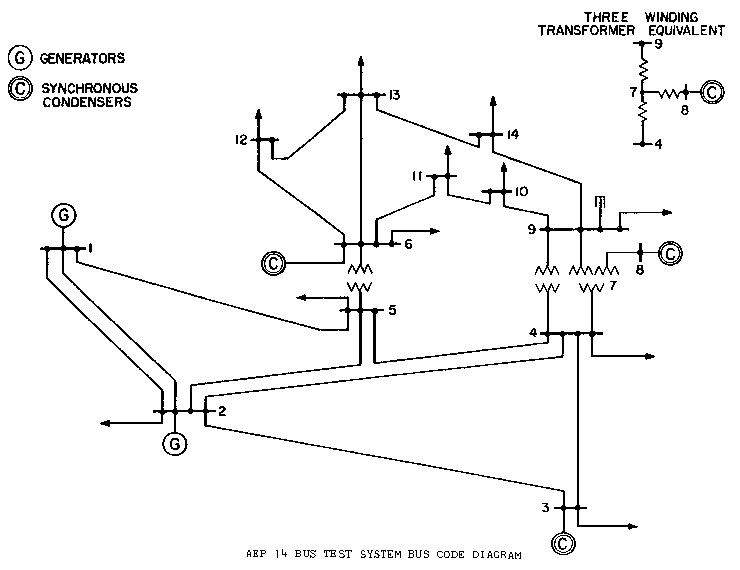
\includegraphics[width=12cm]{figuras/14bus.jpg}
\label{FigRede4barrasLinearizado}
\end{figure}
Neste exercício, será resolvido as tensões e angulos de todas as barras desse sistema, utilizando dados de medições disponíveis na rede. 
\subsection{Dados do Problema}
\label{SectionDados}
Medições do problema \ref{SectionRedePequena}. São dados obtidos da rede que serão usados para estimar o estado do sistema.
\begin{minted}[mathescape, style = autumn,
    frame = single, fontsize=\footnotesize]{matlab}
%         |Msnt |Type | Value | From | To | Rii | 
zdata14   = [ %---- Voltage Magnitude ------------%
            1     1    1.06     1       0   9e-4;
            %-----------------------------------%
            %---- Real Power Injection ---------%
            2     2    0.1830   2       0   1e-4;
            3     2   -0.9420   3       0   1e-4; 
            4     2    0.00     7       0   1e-4;
            5     2    0.00     8       0   1e-4; 
            6     2   -0.0900  10       0   1e-4;
            7     2   -0.0350  11       0   1e-4;
            8     2   -0.0610  12       0   1e-4; 
            9     2   -0.1490  14       0   1e-4;
           %------------------------------------%
           %---- Reative Power Injection -------%
           10     3    0.3523   2       0   1e-4;
           11     3    0.0876   3       0   1e-4; 
           12     3    0.00     7       0   1e-4;
           13     3    0.2103   8       0   1e-4; 
           14     3   -0.0580  10       0   1e-4;
           15     3   -0.0180  11       0   1e-4;
           16     3   -0.0160  12       0   1e-4; 
           17     3   -0.0500  14       0   1e-4;
           %------------------------------------%
           %------ Real Power Flow ------------- %
           18     4    1.5708   1       2   64e-6;
           19     4    0.7340   2       3   64e-6;
           20     4   -0.5427   4       2   64e-6;
           21     4    0.2707   4       7   64e-6;
           22     4    0.1546   4       9   64e-6;
           23     4   -0.4081   5       2   64e-6;
           24     4    0.6006   5       4   64e-6;
           25     4    0.4589   5       6   64e-6;
           26     4    0.1834   6      13   64e-6;
           27     4    0.2707   7       9   64e-6;
           28     4   -0.0816  11       6   64e-6;
           29     4    0.0188  12      13   64e-6;
           %------------------------------------%
           %------ Real Power Flow ------------- %
           30     5   -0.1748   1       2   64e-6;
           31     5    0.0594   2       3   64e-6;
           32     5    0.0213   4       2   64e-6;
           33     5   -0.1540   4       7   64e-6;
           34     5   -0.0264   4       9   64e-6;
           35     5   -0.0193   5       2   64e-6;
           36     5   -0.1006   5       4   64e-6;
           37     5   -0.2084   5       6   64e-6;
           38     5    0.0998   6      13   64e-6;
           39     5    0.1480   7       9   64e-6;
           40     5   -0.0864  11       6   64e-6;
           41     5    0.0141  12      13   64e-6;];
           %--------------------------------------%
\end{minted}

%%%%%%%%%%%%%%%%%%%%%%%%%%%%%%%%%%%%%%%%%%%%%%%
Dados das barras do problema \ref{SectionRedePequena}
\begin{minted}[mathescape, style = autumn,
    frame = single, fontsize=\footnotesize]{matlab}
% |Bus | Type | Vsp | theta | PGi | QGi | PLi | QLi |  Qmin | Qmax |
busdata14 = 
[ 1     1    1.060   0       0     0     0     0       0       0;
  2     2    1.045   0      40   42.4  21.7   12.7    -40     50;
 3     2    1.010   0       0   23.4  94.2   19.0     0      40;
 4     3    1.0     0       0     0   47.8   -3.9     0       0;
 5     3    1.0     0       0     0    7.6    1.6     0       0;
 6     2    1.070   0       0   12.2  11.2    7.5    -6      24;
 7     3    1.0     0       0     0    0.0    0.0     0       0;
 8     2    1.090   0       0   17.4   0.0    0.0    -6      24;
 9     3    1.0     0       0     0   29.5   16.6     0       0;
 10    3    1.0     0       0     0    9.0    5.8     0       0;
 11    3    1.0     0       0     0    3.5    1.8     0       0;
 12    3    1.0     0       0     0    6.1    1.6     0       0;
 13    3    1.0     0       0     0   13.5    5.8     0       0;
 14    3    1.0     0       0     0   14.9    5.0     0       0;];
\end{minted}
Dados dos ramos do problema \ref{SectionRedePequena}
\begin{minted}[mathescape, style = autumn,
    frame = single, fontsize=\footnotesize]{matlab}
%         |  From |  To   |   R     |   X     |     B/2  |  X'mer  |
%         |  Bus  | Bus   |  pu     |  pu     |     pu   | TAP (a) |
linedata14 =[1      2       0.01938   0.05917    0.0264         1
             1      5       0.05403   0.22304    0.0246         1
             2      3       0.04699   0.19797    0.0219         1
             2      4       0.05811   0.17632    0.0170         1
             2      5       0.05695   0.17388    0.0173         1
             3      4       0.06701   0.17103    0.0064         1
             4      5       0.01335   0.04211    0.0            1
             4      7       0.0       0.20912    0.0        0.978
             4      9       0.0       0.55618    0.0        0.969
             5      6       0.0       0.25202    0.0        0.932
             6     11       0.09498   0.19890    0.0            1
             6     12       0.12291   0.25581    0.0            1
             6     13       0.06615   0.13027    0.0            1
             7      8       0.0       0.17615    0.0            1
             7      9       0.0       0.11001    0.0            1
             9     10       0.03181   0.08450    0.0            1
             9     14       0.12711   0.27038    0.0            1
            10     11       0.08205   0.19207    0.0            1
            12     13       0.22092   0.19988    0.0            1
            13     14       0.17093   0.34802    0.0            1 ];
\end{minted}

\section{Resultado do Estimador de Estados}
\label{SectionResultados}
Os resultados das duas soluções convergiram para esse problema. Nota-se que o tempo computacional utilizando Tableau Esparso é menor, embora a comparação tenha apenas efeito didático já que o processador não é dedicado e pode variar o tempo de solução.

\subsection{Equação Normal}
Aqui, a matriz $G$ foi calculada como em \ref{G}. O código está na seção \ref{SectionEqNormal}
\begin{minted}[mathescape, style = autumn,
    frame = single, fontsize=\footnotesize]{matlab}
    
-------- State Estimation ------------------
--------------------------
| Bus |    V   |  Angle  | 
| No  |   pu   |  Degree | 
--------------------------
   1    1.0068     0.0000
   2    0.9899    -5.5265
   3    0.9518   -14.2039
   4    0.9579   -11.4146
   5    0.9615    -9.7583
   6    1.0185   -16.0798
   7    0.9919   -14.7510
   8    1.0287   -14.7500
   9    0.9763   -16.5125
  10    0.9758   -16.7476
  11    0.9932   -16.5397
  12    1.0009   -17.0203
  13    0.9940   -17.0583
  14    0.9647   -17.8967
---------------------------------------------
Tempo computacional =  0.0834 segundos.
\end{minted}
\subsection{Tableau Esparso}
Aqui, a matriz $G$ não foi calculada. O calculo foi feito como em \ref{EQ_Tableau}. O código está na seção \ref{SectionTableau}
\begin{minted}[mathescape, style = autumn,
    frame = single, fontsize=\footnotesize]{matlab}
    
-------- State Estimation ------------------
-------- Tableau Sparse   ------------------
--------------------------
| Bus |    V   |  Angle  | 
| No  |   pu   |  Degree | 
--------------------------
   1    1.0068     0.0000
   2    0.9899    -5.5265
   3    0.9518   -14.2039
   4    0.9579   -11.4146
   5    0.9615    -9.7583
   6    1.0185   -16.0798
   7    0.9919   -14.7510
   8    1.0287   -14.7500
   9    0.9763   -16.5125
  10    0.9758   -16.7476
  11    0.9932   -16.5397
  12    1.0009   -17.0203
  13    0.9940   -17.0583
  14    0.9647   -17.8967
---------------------------------------------
Tempo computacional =  0.0469 segundos.
\end{minted}